\documentclass[a4paper, 12pt, oneside]{book}
\usepackage[utf8]{inputenc}
\usepackage[margin=3cm, bindingoffset=1cm]{geometry}
\linespread{1.5}
\usepackage[backend=biber, sorting=none]{biblatex}
\addbibresource{bib.bib}
\usepackage{float}
\usepackage{csquotes}
\usepackage{subfig}
\usepackage{graphicx}
%\usepackage{indentfirst}
\usepackage{fancyhdr}
\usepackage{xcolor}
\usepackage[acronym]{glossaries}
\usepackage{comment}
\makenoidxglossaries
\newacronym{er}{ER}{Emotion Recognition}
\newacronym{fer}{FER}{Facial Emotion Recognition}
\newacronym{ser}{SER}{Speech Emotion Recognition}
\newacronym{ml}{ML}{Machine Learning}
\newacronym{anns}{ANNs}{Artificial Neural Networks}
\newacronym{cnn}{CNNs}{Convolutional Neural Networks}
\newacronym{rnn}{RNNs}{Recurrent Neural Networks}
\newacronym{asr}{ASR}{Automatic Speech Recognition}
\newacronym{ai}{AI}{Artificial Intelligence}
\newacronym{hci}{HCI}{Human-Computer Interaction}
\newacronym{crnn}{CRNN}{Convolutional Recurrent Neural Network}


\setlength{\parindent}{1cm}

\pagestyle{fancy}
\renewcommand{\chaptermark}[1]{\markboth{\thechapter.\ \uppercase{#1}}{}}
\fancyhf{}
\fancyhead[C]{\textbf{\leftmark}}
\fancyfoot[C]{\thepage}
\renewcommand{\headrulewidth}{1pt}
\renewcommand{\footrulewidth}{1pt}
\usepackage[Conny]{fncychap}
%\usepackage[style=ieee]{biblatex}

\title{Tesi Magistrale}
\author{Ivan Colucci}
\date{January 2020}

\newenvironment{dedication}
  {\clearpage           % we want a new page
   \thispagestyle{empty}% no header and footer
   \vspace*{\stretch{1}}% some space at the top 
   \itshape             % the text is in italics
   \raggedleft          % flush to the right margin
  }
  {\par % end the paragraph
   \vspace{\stretch{3}} % space at bottom is three times that at the top
   \clearpage           % finish off the page
  }

\graphicspath{{images/}}
  
\begin{document}
%Frontespizio
\begin{titlepage}
    \begin{center}
        \LARGE{\uppercase{Università degli Studi di Salerno}}\\
        \vspace{5mm}
        %Dipartimento
    	\uppercase{\normalsize Dipartimento di Ingegneria del informatica }\\
    \end{center}
    \begin{figure}[H]
        \centering
        
\includegraphics[width=0.25\textwidth]{logo_unisa}
    \end{figure}
    
    \begin{center}
        %Corso di Laurea
    	\normalsize{Project in Software Engineering for Artificial intelligence}\\
    	\vspace{15mm}
    	%Titolo
        {\LARGE{\bf Experimenting with Emotional Recognition Systems}}\\
    	\vspace{3mm}
    \end{center}
    
    \vspace{7mm}
    \noindent
    \begin{center}
        %Relatore
    	{\large{ Authors:\\\bf John Carlsson, 
                 Philip Le Borne, \\
                 Sarah Ternus,
                 Lukas Runt,\\
                 Cyprien Touron Decourteix,\\
                 Jana Valentina Stefan,\\
                 Simon Dannemann,\\
                 Ergi Kokoshi}}
    	\vspace{12mm}\\
    
    \url{https://github.com/John-Carlsson/SE4AI}
    	
    \end{center}
    
    \hfill
    
    %Anno Accademico
    \centering{\large \uppercase{ Anno Accademico 2022/2023 }}

\end{titlepage}
\begin{dedication}
Dedicata a coloro che\\ ci provano ogni giorno.
\end{dedication}
%Corpo della Tesi

\tableofcontents
\thispagestyle{empty}
\clearpage

\pagenumbering{Roman}\thispagestyle{empty}
\addcontentsline{toc}{chapter}{Acronyms}
\printnoidxglossary[type=\acronymtype,title=Acronyms,nonumberlist]
\newpage 
\listoffigures
\addcontentsline{toc}{chapter}{\listfigurename}
\clearpage
%\listoftables
%\addcontentsline{toc}{chapter}{\listtablename}

%\sloppy
%\hyphenpenalty=10000
%\exhyphenpenalty=10000

\newcounter{savepage}
\setcounter{savepage}{\arabic{page}}
\pagenumbering{arabic}

%\chapter{Timeplan and Work Distribution}
%\begin{table}[]
    \centering
    \begin{tabular}{c|c}
         &  \\
         & 
    \end{tabular}
    \caption{Timeplan}
    \label{tab:timeplan}
\end{table} 

\chapter{Introduction} \label{chap:introduction}
 \noindent The field of \acrfull{er} has grown in importance as \acrfull{ai} and \acrfull{ml} have gained popularity due to its potential to transform a variety of fields and applications \cite{er-appl}. With the ongoing evolution of virtual environments, such as the Metaverse, \acrshort{er} is gaining momentum as a critical component in creating a more immersive and engaging experience. By utilizing AI algorithms to analyze various physiological responses and facial expressions, \acrshort{er} technology has the potential to enhance social interactions and emotional experiences of users in virtual environments. But not only that, \acrshort{er} can offer great benefits in many other fields as well, such as marketing, healthcare, education and \acrfull{hci} \cite{er-appl,healthcare,EGGER201935}. As a contribution to this change, our project aims to develop a system that recognizes emotions based on both facial and speech features. Firstly, we examine what approaches have been taken so far in chapter \ref{chap:related-work}. Then, in chapter \ref{chap:project-ideas}, we define our idea and the resulting goals in more detail. In chapter \ref{chap:methodology}, we address the methodology to achieve those goals. In this context, we will observe our approach for \acrfull{fer} and \acrfull{ser} seperately. Moreover, in the course of the project we will address the the discussed steps and implementation in more detail.


\chapter{Related Work} \label{chap:related-work}
\begin{figure}[h]
\centering
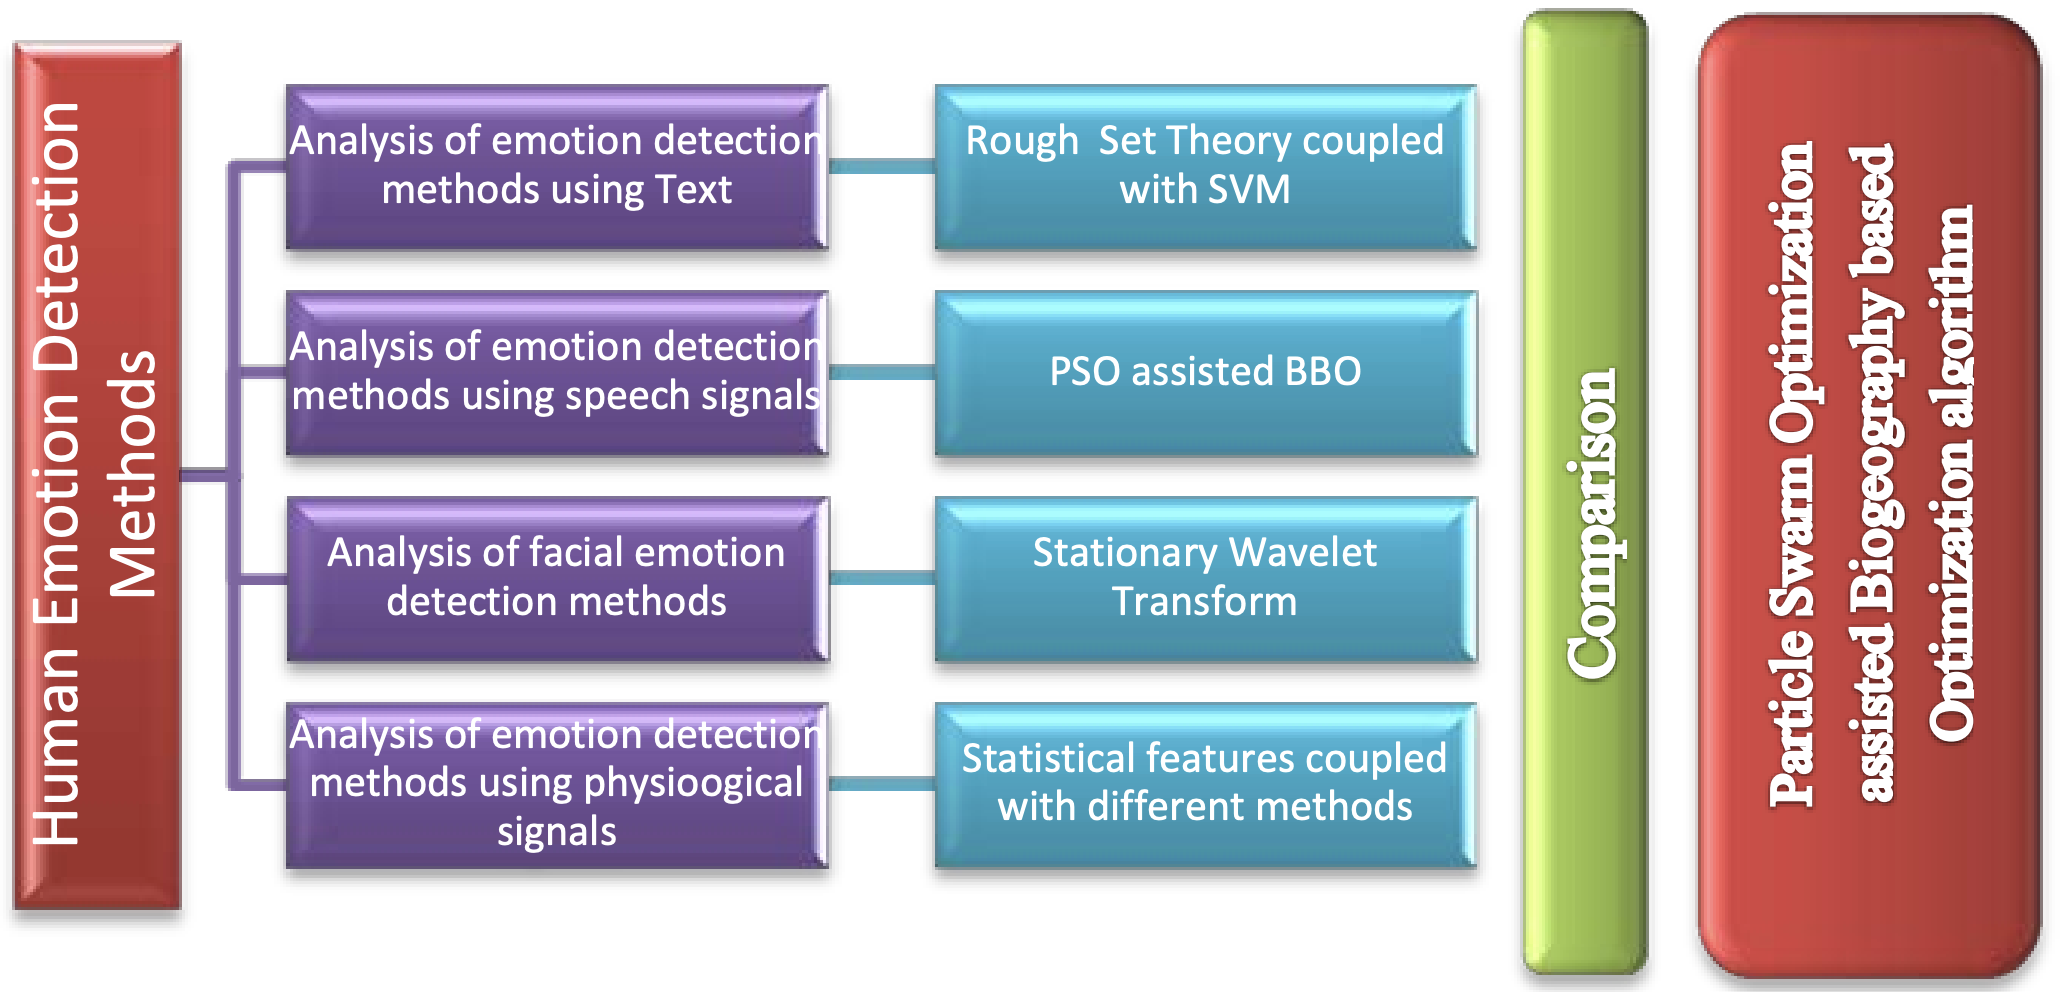
\includegraphics[width=1\textwidth]{images/Emotion-detection-survey.png}
\caption{Survey on Emotional Detection. \cite{survey}}\label{fig:survey}
\end{figure}

\noindent The current work on emotional recognition is an active and rapidly developing field with many applications as already touched upon in chapter \ref{chap:introduction}. Like figure \ref{fig:survey} shows, there are many possibilities to approach this. Continuing, we will focus on \acrshort{fer} and \acrshort{ser}.\\

\noindent \acrshort{fer} is an important area of research that has many applications in \acrshort{hci} and other fields. \acrfull{cnn} have emerged as a promising approach for \acrshort{fer}, but there are numerous factors that can impact their performance. As of today, there are multiple state-of-the-art \acrshort{cnn}-based \acrshort{fer} methods that differ in their architecture, preprocessing, and training/test protocols, of which \cite{pramerdorfer2016facial} analyzed six.

\noindent Especially recognizing facial expressions under naturalistic conditions is still an unsolved problem and represents a great challenge. One way to improve \acrshort{fer} performance is to overcome the bottleneck of using comparatively basic CNN architectures. A collection of modern \acrshort{cnn} has achieved a FER2013 \cite{FER2013} test accuracy of 75.2\%, outperforming previous works without requiring auxiliary training data or face registration \cite{pramerdorfer2016facial}.

\noindent In the area of \acrshort{ser} the research is ongoing. Also, in the specific branch of \acrshort{hci} \acrshort{cnn} are commonly used for feature extraction and classification in \acrshort{ser}. Besides, \acrfull{rnn} (especially Gated Recurrent Unit architectures) are also effective methods for emotion recognition through speech. In this case the highest accuracy scored was 97.47\% was \cite{GRU}.

\noindent It is also interesting to have a look at the transformer-based models, which recently were used for \acrshort{ser} with promising results \cite{transform}. \acrshort{ser} under realistic conditions presents several challenges, including the variability in speech patterns and background noise.


% Quelle: https://www.mdpi.com/1424-8220/22/4/1414#:~:text=The%20data%20augmentation%20was%20used,average%20recognition%20accuracy%20of%2097.47%25.

%https://deepai.org/machine-learning-glossary-and-terms/gated-recurrent-unit

%https://www.nature.com/articles/s41598-022-12260-y

\chapter{Project Idea and Goals} \label{chap:project-ideas}
\noindent The project idea is to use \acrshort{ml} algorithms that can recognize emotions in facial images and speech. The system will be developed using software engineering principles such as modular design, testing, and documentation to ensure reliability, scalability, and maintainability. The system will also incorporate user feedback mechanisms to improve accuracy and adaptability to new scenarios. \\

\noindent As discussed the previous chapters, there are plenty of areas in which such a solution can be used. It has then become a challenging problem that this field involves more and more scientists with different specializations \cite{HCSI201451}. %This project aims to create a viable solution that serves as a first step towards a complete solution in a real life problem. \newpage %not true & doubled at next page
\\\\
\noindent The goal of the project is to create a viable, working application that can differentiate between emotions using pictures or possibly a video and vocal sound of the user. Thereby, recognizing emotion via speech follows two approaches: 
\begin{enumerate}
    \item using \emph{phonological} information (pitch, amplitude, spectral features, etc.)
    \item using \emph{semantic} information (words, grammar)
\end{enumerate}
\newpage
\noindent More specifically, the goals are as follows:

\begin{itemize}

    \item Create a model that achieves a classification accuracy of 80\% on the given dataset, this can be achieved by grouping the emotions into wider groups, such as positive or negative and 60\% for a more detailed differentiation in emotions
    \item Make a working application that can handle new inputs.
    \item Implement a small GUI including a feedback mechanism for the users, which should follow the user experience and the usability principles by showing emojis or a bar chart where the user can specify their emotions. Due to time constraints, it will be kept simple. 
    \item Possibly combine the two approaches and analyse the pros and cons of this combined approach
\end{itemize}

\noindent More information about each approach is available in the methodology chapter.
\\

\begin{comment}
\noindent
We will follow two approaches to recognize emotion in speech: 
\begin{enumerate}
    \item using \emph{phonological} information (pitch, amplitude, spectral features, etc.)
    \item using \emph{semantic} information (words, grammar)
\end{enumerate}
\noindent
The working system should then follow this procedure:
\begin{enumerate}
    \item Take in a continuous audio stream
    \item Cut it into samples every $x$ seconds
    \item Preprocess the samples
    \item Feed the samples to the neural network models
    \item Publish classification results continuously 
    \item At the same time: show user interface to obtain feedback
    \item Incorporate user feedback
\end{enumerate}
\end{comment}









\chapter{Methodology} \label{chap:methodology}
\input{texts/methodology}

%\chapter{Implementation} \label{chap:Implementation}

%\chapter{Conclusion}\label{chap:conclusion}
%\input{texts/conclusion}
\cleardoublepage
\pagenumbering{Roman}
\setcounter{page}{\thesavepage}
\printbibliography[heading=bibintoc,title={References}]
\clearpage
%\clearpage
\end{document}
